Após conversas com a cliente e com a solicitante do software, foi possível identificar quatro módulos principais que contemplam as diferentes funcionalidades solicitadas. Estes módulos são apresentados a seguir:

\begin{enumerate}
	\item \textbf{Módulo Gerencia Conta de Usuário}. Neste módulo, cujo ator principal é o administrador do sistema, concentram-se as funcionalidades relativas à manutenção de usuários, ilustradas no diagrama de caso de uso da Figura \ref{fig:casoUso1}. No cenário em que a plataforma será utilizada, foi possível identificar que não deve haver livre cadastro e acesso aos dados de maneira deliberada, daí a necessidade de um administrador para cadastrar novos usuários, que podem ser alunos de iniciação científica, pesquisadores, docentes, dentre outros;
	\begin{figure}[H]
		\centering
		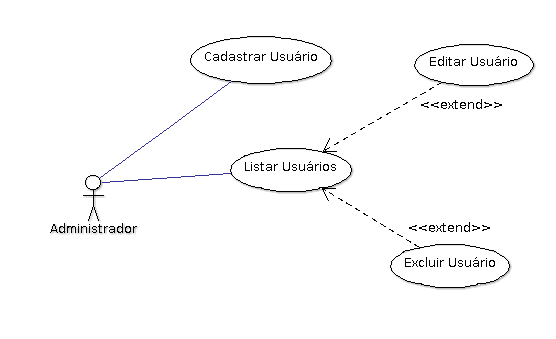
\includegraphics[scale=0.8]{img/uc001.png}
		\caption{Caso de Uso - Módulo Gerencia Conta de Usuário.}
		\label{fig:casoUso1}
	\end{figure}
	\item \textbf{Módulo Usuário}. Neste módulo, cujo ator principal é o usuário, encontram-se as funcionalidades relativas à manutenção dos dados do próprio usuário. Pode haver alterações de dados do perfil, redefinição e recuperação de senha, conforme ilustrado na Figura \ref{fig:casoUso2};
	\begin{figure}[H]
		\centering
		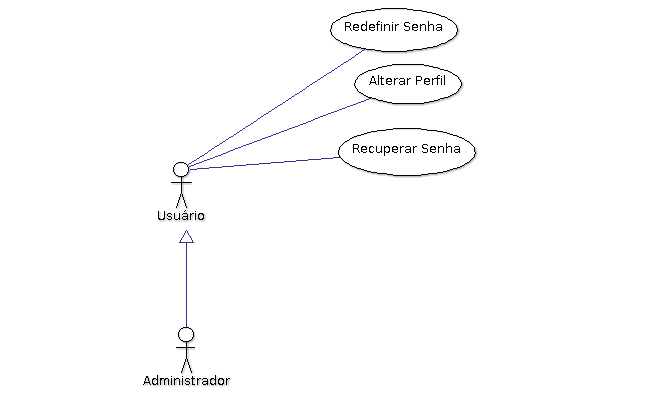
\includegraphics[scale=0.8]{img/uc002.png}
		\caption{Caso de Uso - Módulo Usuário.}
		\label{fig:casoUso2}
	\end{figure}
	\item \textbf{Módulo Consulta Medições}. Este módulo concentra as funcionalidades de acesso aos dados das estações. Conforme ilustra a Figura \ref{fig:casoUso3}, podem ser feitas consultas diretas aos dados, consulta à disponibilidade dos dados em um determinado mês e também aspectos da visualização dos dados, seja por meio de boletins como também por meio de gráficos, além da possibilidade de exportação. Estas funcionalidades foram identificadas considerando as principais solicitações de dados feitas por terceiros ao LabInstru;
	% figura 3
	\begin{figure}[H]
		\centering
		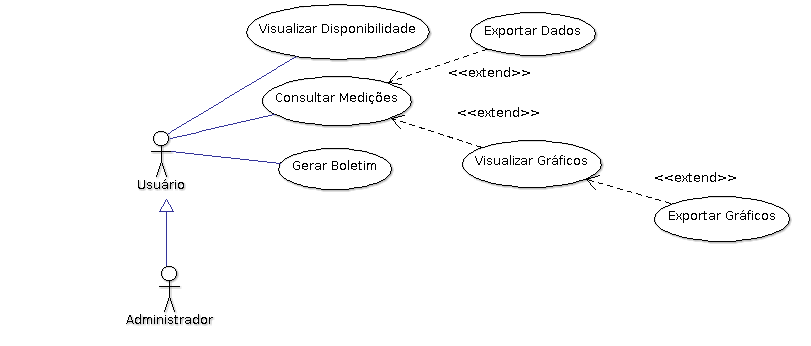
\includegraphics[scale=0.8]{img/uc003.png}
		\caption{Caso de Uso - Módulo Consulta Medições.}
		\label{fig:casoUso3}
	\end{figure}
	\item \textbf{Módulo Gerencia Medições}. O módulo de gerenciamento de medições permite que o administrador do sistema mantenha as medições do sistema a partir dos dados obtidos das estações meteorológicas do LabInstru. Considerando a importância de assegurar a origem destes dados e a remoção das eventuais medições inconsistentes, apenas o administrador está habilitado para execução das funcionalidades deste módulo, conforme ilustrado na Figura \ref{fig:casoUso4}.
	% figura 4
	\begin{figure}[H]
		\centering
		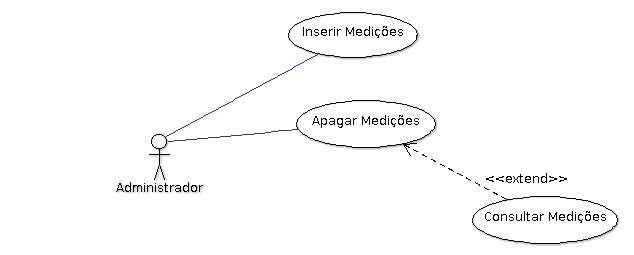
\includegraphics[scale=0.8]{img/uc004.png}
		\caption{Caso de Uso - Módulo Gerencia Medições.}
		\label{fig:casoUso4}
	\end{figure}
\end{enumerate}

O detalhamento de todos os casos de uso ilustrados nas Figuras \ref{fig:casoUso1}-\ref{fig:casoUso4} encontra-se disponível no Apêndice \ref{sec:aprendiceCasoUso},  onde podem ser vistos os interessados, pré e pós condições, fluxo principal, fluxo alternativo e regras de negócio.
